\documentclass[preprint,12pt,authoryear]{elsarticle}

\usepackage{amsmath,amssymb,amsthm}
\usepackage{booktabs}
\usepackage{graphicx}
\usepackage{xcolor}
\usepackage[ruled,vlined,linesnumbered]{algorithm2e}
\SetKwProg{Fn}{function}{}{}
\SetKw{Break}{break}
\SetKwFor{ForR}{for}{do}{}
\usepackage{hyperref}

% numeros provisionales (se reemplazan con la corrida final: 10 semillas, mismo tiempo, version final)
\newcommand{\prov}[1]{\textcolor{blue}{#1}}
\newcommand{\todo}[1]{\textcolor{red}{[TODO: #1]}}

\newtheorem{proposition}{Proposition}
\newtheorem{definition}{Definition}

\journal{European Journal of Operational Research}

\begin{document}

\begin{frontmatter}

\title{Fast exact overlap minimization for three-dimensional irregular strip packing of polyhedra}

\author[pucv]{Ignacio Araya\corref{cor1}}
\ead{ignacio.araya@pucv.cl}
\cortext[cor1]{Corresponding author}
\address[pucv]{Escuela de Ingenier\'ia Inform\'atica, Pontificia Universidad Cat\'olica de Valpara\'iso, Chile}
% TODO: coautores y afiliaciones

\begin{abstract}
We address the three-dimensional irregular strip packing problem: polyhedra, possibly non-convex, must be placed
by translation in a container with a fixed rectangular base so that the height is minimized. We propose an
overlap-minimization heuristic that works with the exact geometry of the pieces, represented as unions of convex
parts. Its main ingredient is an exact axis move. The overlap of two parts is measured by the penetration depth
of their relative position in their no-fit polytope; along any axis this function is zero outside an interval
and concave inside it, so the best position of a piece along an axis is found by evaluating a few breakpoints
only. The move is embedded in a strategic oscillation of the container height with guided local search weights
and restarts, starting from a greedy construction and a linear-programming compaction. On the benchmarks of
polyhedral pieces, the method improves the best known heights of 11 of 13 instances within two minutes, reaches
in 10 seconds the quality that the previous exact local search attains in 600 seconds, and matches 26 of the 27
known optima of small instances. An ablation study shows that the speed of the move and the guided local search
weights are the decisive components.
\end{abstract}

\begin{keyword}
Cutting \sep Packing \sep 3D irregular packing \sep No-fit polytope \sep Guided local search \sep Linear programming
\end{keyword}

\end{frontmatter}

% =====================================================================================================
\section{Introduction}

Three-dimensional irregular packing arises in additive manufacturing (packing parts in the build volume of a
printer), in the loading of non-rectangular goods, and in the design of compact assemblies. In its open-dimension
variant, the \emph{3D irregular strip packing problem}, a set of polyhedra must be placed without overlap inside
a container with a fixed $W\times D$ base, and the height of the packing is to be minimized. We consider the
translational version: pieces keep their orientation.

The literature on this problem is small compared with its two-dimensional counterpart, and it is split by the
representation of the geometry. Exact approaches use the polyhedra directly: phi-functions and nonlinear
programming \citep{stoyan2004,stoyan2005,romanova2018}, the 3DNest local search of \citet{egeblad2009}, which
minimizes the exact overlap volume along axis-parallel translations, constructive heuristics such as HAPE3D
\citep{liu2015}, and, recently, mixed-integer models based on no-fit polyhedra that solve small convex instances
to optimality \citep{tollenaere2026}. Approximate approaches discretize the pieces into voxels
\citep{lamas2023}; voxels make overlap tests trivial and scale well, but they overestimate the pieces and the
quality of the solutions depends on the resolution.

In two dimensions, the most successful methods for irregular strip packing are overlap-minimization heuristics:
the height (length) is decreased, the pieces are allowed to overlap, and a local search moves them until the
overlap vanishes \citep{egeblad2007,umetani2009,imamichi2009,elkeran2013,gardeyn2025}. The key ingredients are a
cheap and informative overlap measure, moves that can be optimized exactly or quickly, and guided local search
(GLS) weights to escape local minima. This paper brings these ingredients to three-dimensional polyhedra with an
exact representation.

\paragraph{Contributions}
\begin{enumerate}
\item An exact and fast overlap-minimization move for polyhedra represented as unions of convex parts. Overlap
is measured by the penetration depth in the NFP of each pair of convex parts; along an axis this function is
concave on an interval and zero outside it, so the optimal position of a piece along an axis is attained at an
interval endpoint (Proposition~\ref{prop:axis}). The move extends the directional moves of
\citet{umetani2009} to 3D and non-convex pieces and is much cheaper than the exact overlap volume of
\citet{egeblad2009}.
\item A strategic oscillation with multiplicative GLS weights \citep{gardeyn2025} and restarts, and an ablation
study showing that the weights and the speed of the separation are decisive, whereas a global LP compaction over
NFP facets, in the spirit of \citet{gomes2006} in 2D, has no measurable effect on the quality.
\item New best known solutions on the Merged instances of \citet{egeblad2009} and on classical instances of
\citet{stoyan2004,stoyan2005}, with a time-matched comparison against the exact method 3DNest, and a comparison
with the optimal values and bounds of the mixed-integer models of \citet{tollenaere2026}.
\item An exact convex decomposition of the non-convex (prismatic) pieces of \citet{ikonen1997} used in the
Merged instances.
\end{enumerate}

Section~\ref{sec:problem} defines the problem and the geometric tools. Section~\ref{sec:method} describes the
algorithm, and Section~\ref{sec:exp} the experiments.

% =====================================================================================================
\section{Problem and geometry}\label{sec:problem}

\subsection{Problem}
We are given a container base $W\times D$ and $n$ pieces $P_1,\dots,P_n$ (polyhedra, with multiplicities). Each
piece is a union of convex polytopes, $P_i=\bigcup_{a\in\mathcal{A}_i}A_a$, expressed in a local frame where the
minimum of its bounding box is the origin; $w_i,d_i,h_i$ denote its bounding-box dimensions. A solution is a
vector of translations $t_i=(x_i,y_i,z_i)$ such that
\begin{align}
& 0\le x_i\le W-w_i,\quad 0\le y_i\le D-d_i,\quad z_i\ge 0, && i=1,\dots,n,\\
& \operatorname{int}(P_i+t_i)\cap\operatorname{int}(P_j+t_j)=\emptyset, && i<j,
\end{align}
where $\operatorname{int}(\cdot)$ denotes the interior of a set (pieces may touch but not overlap), and the
objective is to minimize $H=\max_i(z_i+h_i)$. A trivial lower bound is
$H_0=\max\{\max_i h_i,\ \sum_i\operatorname{vol}(P_i)/(WD)\}$.

\subsection{No-fit polytopes and penetration depth}
For two convex parts $A$ and $B$ placed at $t_A$ and $t_B$, their interiors intersect if and only if the relative
position $r=t_A-t_B$ lies in the interior of the no-fit polytope
\begin{equation}
N_{AB}=B\oplus(-A)=\operatorname{conv}\{b-a:\ a\in V(A),\ b\in V(B)\},
\end{equation}
where $V(\cdot)$ is the vertex set \citep{bennell2008}. We compute $N_{AB}$ once per pair of parts as the convex
hull of the vertex differences and store it in H-representation, $N_{AB}=\{r:\ n_f\cdot r\le d_f,\ f\in F_{AB}\}$,
with unit normals $\|n_f\|=1$.

\begin{definition}
The \emph{penetration} of $A$ and $B$ at relative position $r$ is
$\delta_{AB}(r)=\max\{0,\ \min_{f\in F_{AB}}(d_f-n_f\cdot r)\}$.
\end{definition}

For $r$ inside $N_{AB}$, $\delta_{AB}(r)$ is the Euclidean distance from $r$ to the boundary of $N_{AB}$, i.e.,
the length of the shortest translation that separates $A$ and $B$, known as the translational penetration
depth \citep{cameron1986,agarwal2000}. It is
zero if and only if the parts do not overlap. For two pieces we use
$\delta_{ij}(t_i-t_j)=\sum_{a\in\mathcal{A}_i}\sum_{b\in\mathcal{A}_j}\delta_{ab}(t_i-t_j)$, where only pairs of parts
whose bounding boxes intersect are evaluated. Figure~\ref{fig:nfp} illustrates both definitions in two dimensions.

\begin{figure}[!tbp]
\centering
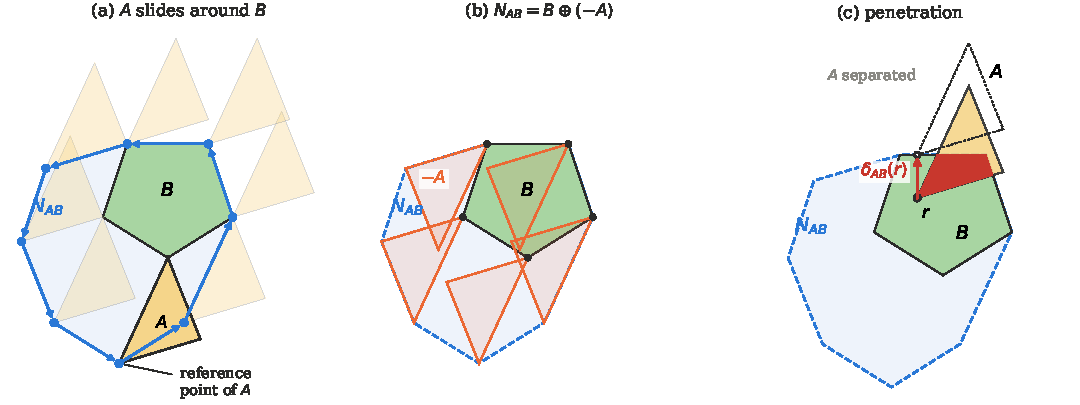
\includegraphics[width=\textwidth]{figures/nfp.pdf}
\caption{No-fit polytope and penetration in 2D. (a) When $A$ slides around $B$ keeping contact, its reference
point (the minimum of its bounding box) traces the boundary of $N_{AB}$; the shaded copies of $A$ touch $B$ at the
vertices of $N_{AB}$. (b) Equivalently, $N_{AB}=B\oplus(-A)$ is the convex hull of the copies of $-A$ placed at the
vertices of $B$. (c) If $r$ lies inside $N_{AB}$ the parts overlap (red), and $\delta_{AB}(r)$ is the distance
from $r$ to the nearest facet: the shortest translation of $A$ that separates the parts (dotted).}
\label{fig:nfp}
\end{figure}

\subsection{Exact minimization along an axis}
Let all pieces but $i$ be fixed, and let $i$ move along axis $e_k$, $t_i(s)=t_i+(s-t_{ik})e_k$, with
$s\in[0,U_k]$ (the container limits, using the current height $H$ for the vertical axis). The weighted overlap
of $i$ is
\begin{equation}\label{eq:obj}
\phi(s)=\sum_{j\ne i}w_{ij}\,\delta_{ij}\big(t_i(s)-t_j\big),
\end{equation}
where the weights $w_{ij}\ge 1$ (initially 1) are the penalties of guided local search (GLS)
\citep{voudouris1999}: they are increased for the pairs that remain overlapping at local minima, so that the
search focuses on them (Section~\ref{sec:minover}).

\begin{proposition}\label{prop:axis}
Each term $\delta_{ab}(t_i(s)-t_j)$ is zero outside an interval $(L_{ab},U_{ab})$ and concave inside it. Hence
$\phi$ is concave on every interval between consecutive points of
$\mathcal{B}=\{0,U_k\}\cup\{L_{ab},U_{ab}\}$, and a minimizer of $\phi$ on $[0,U_k]$ is attained at a point of
$\mathcal{B}$.
\end{proposition}
\begin{proof}
Along the line, $d_f-n_f\cdot r(s)=c_f-n_{fk}s$ is affine. The set where all of them are positive is the open
interval $(L_{ab},U_{ab})$ with $L_{ab}=\max_{n_{fk}<0}c_f/n_{fk}$ and $U_{ab}=\min_{n_{fk}>0}c_f/n_{fk}$
(facets with $n_{fk}=0$ only decide whether the interval is empty). Inside it, $\delta_{ab}$ is a minimum of
affine functions, hence concave; outside it is zero. Between consecutive points of $\mathcal{B}$ every term is
either concave or identically zero, so $\phi$ is concave there and attains its minimum at an endpoint.
\end{proof}

Figure~\ref{fig:axis} illustrates the proposition in two dimensions.

\begin{figure}[!tbp]
\centering
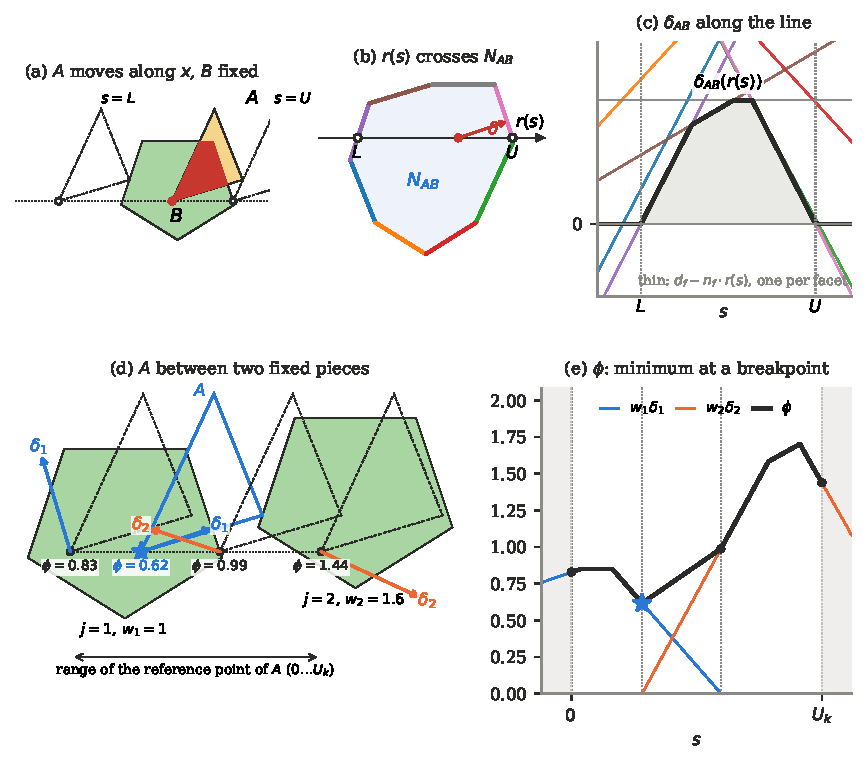
\includegraphics[width=\textwidth]{figures/axis.pdf}
\caption{Proposition~\ref{prop:axis} in 2D, with the parts of Figure~\ref{fig:nfp}. (a) Part $A$ moves along
$x$ with $B$ fixed: it touches $B$ at $s=L$ and $s=U$ (dashed) and overlaps it in between (red). (b) In the space of
relative positions, $r(s)$ moves along a line that enters $N_{AB}$ at $L$ and leaves it at $U$. (c) For each
facet (same colors as in (b)), $d_f-n_f\cdot r(s)$ is affine in $s$; the penetration is the lower envelope of these
lines clipped at zero: zero outside $(L,U)$ and concave inside. (d)--(e) $A$ moves between two fixed pieces within
the container range $[0,U_k]$. In (d), $A$ is drawn at each breakpoint of (e) ($0$, $U_k$ and the $L$, $U$ of
each term; dots: its reference point), with arrows for its penetration with each piece it overlaps ($\delta_1$,
$\delta_2$) and the resulting $\phi=w_1\delta_1+w_2\delta_2$ (weights $w_1=1$, $w_2=1.6$): the two central
positions have similar penetrations but different $\phi$. Between consecutive breakpoints the weighted overlap $\phi$ is a sum of concave functions, so its
minimum (star, solid outline in (d)) is at a breakpoint, and only these points are evaluated.}
\label{fig:axis}
\end{figure}

The move evaluates $\phi$ at the points of $\mathcal{B}$ only. With the interval of each term known, a term is
evaluated only at the candidates inside it: sorting the candidates, each term contributes to a contiguous range
found by binary search. Facets are stored as $(c_f,n_{fk})$ in contiguous arrays, so evaluating a term costs one
fused multiply-add per facet. Ties are broken towards the smaller coordinate (gravity and walls).

% =====================================================================================================
\section{Algorithm}\label{sec:method}

Algorithm~\ref{alg:main} summarizes the method. A greedy construction and an LP compaction give a first feasible
solution $S$ of height $H$. The search then tries to fit the pieces in a slightly lower container: the
positions of $S$ are \emph{clamped} to a target height $h<H$: \textsc{Clamp}($S,h$) moves every piece that
exceeds $h$ down until its top is at $h$, regardless of the other pieces. This is where overlaps appear, and
\textsc{MinimizeOverlap} tries to remove them. If it succeeds, the layout is feasible again: it is compacted, it
becomes the new best solution, and the target is lowered; otherwise the target is raised slightly and, when it
reaches $H$, the search restarts from the best solution.

\begin{algorithm}[t]
\caption{Overview}\label{alg:main}
\SetCommentSty{textit}
$S\gets$ \textsc{Greedy}(); $S\gets$ \textsc{Compact}($S$); $H\gets H(S)$\;
$h\gets(1-\rho)H$; $T\gets$ \textsc{Clamp}($S,h$); $w\gets 1$\tcp*{overlaps appear}
\While{time remains}{
  \eIf(\tcp*[f]{$T$ is feasible}){\textsc{MinimizeOverlap}($T,h,w$)}{
    $T\gets$ \textsc{Compact}($T$)\;
    \lIf{$H(T)<H$}{$S\gets T$; $H\gets H(T)$}
    $h\gets(1-\rho)H$; $T\gets$ \textsc{Clamp}($S,h$); $w\gets 1$\;
  }{
    $h\gets h+\rho H/4$; $T\gets$ \textsc{Clamp}($T,h$)\tcp*{keeps the overlaps}
    \If{$h\ge H$}{
      $h\gets(1-\rho)H$; $T\gets$ \textsc{Clamp}($S,h$); move a random piece of $T$; $w\gets 1$\tcp*{restart}
    }
  }
}
\Return $S$\;
\end{algorithm}

In Algorithm~\ref{alg:main}, line~1 builds the first solution (Sections~\ref{sec:greedy} and~\ref{sec:compact}) and
line~2 creates the first overlapping layout. Each iteration of the loop is a separation attempt at height $h$
(Section~\ref{sec:minover}). On success (lines~5--7) the separated layout is compacted, possibly becomes the new
best solution, and the target is lowered again from the best height. On failure (lines~9--11) the target is raised
by a quarter of the step and the search continues from the current overlapping layout with the current weights;
once the target is back at the best height, the search restarts from the best solution
(Section~\ref{sec:kicks}).

\subsection{Greedy construction}\label{sec:greedy}
Pieces are placed one at a time on top of the current load (Algorithm~\ref{alg:greedy}). For each type of piece
still to be placed, $g\times g$ starting points ($g=4$) are taken on a regular grid of the base, at the current
height $H_{\text{cur}}$ of the load, and from each of them the piece descends (\textsc{Descend}, lines~9--18).
The descent is a sequence of small linear programs in the three translation variables of the piece. At the
current point $t$, for every placed part $b$ that the part $a$ of the piece may meet within a trust region (a box
of half side $\Delta$, the largest dimension of the piece), one facet of $N_{ab}$ satisfied at $t$ is selected:
the one that allows the longest step in the descent direction (line~13). The selected facets define a convex
region of positions where the piece does not overlap the placed parts, and the LP of line~14 minimizes
$c\cdot u=z+\sigma\,\mathrm{dist}_{\text{wall}}(x,y)$ in it: the piece goes down and, with a small weight $\sigma$,
towards the nearest walls in $x$ and $y$. The facets are re-selected at the new point and the procedure stops
when the objective no longer decreases. Figure~\ref{fig:descend} shows the LPs of one descent.

Among all piece types and resulting positions, the greedy places the pair $(k,t)$ that maximizes (line~6)
\begin{equation}\label{eq:greedy}
\mathit{val}(k,t)=\alpha\log\frac{V_k}{V_{\max}}-\beta\,\frac{z}{H_0}-\gamma\,\frac{\max(0,\,z+h_k-H_{\text{cur}})}{H_0},
\end{equation}
where $V_k$ is the volume of the piece, $V_{\max}$ the largest volume, $z$ the height of the position and
$H_{\text{cur}}$ the current height of the load. The first term favors large pieces, as the classical orderings by
decreasing volume, but on a logarithmic scale, so that a smaller piece is preferred when it fits clearly lower.
The second term favors low positions, i.e., filling the gaps of the load before building on top of it, and the
third penalizes positions that raise the height of the load. Normalizing by the lower bound $H_0$ makes the
parameters independent of the scale of the instance. For a given piece the score decreases with $z$, so the
lowest of its positions is always preferred; the score thus decides which piece is placed next: a large piece
if it fits in a low gap, and a smaller one if the large pieces would raise the height. The parameters
($\alpha=1$, $\beta=5.53$, $\gamma=0.77$, $\sigma=0.065$) were tuned with Optuna on 16 training instances, for an
earlier version of the method that relied more on the construction. Figure~\ref{fig:construction} illustrates
the construction in two dimensions.

\begin{algorithm}[!htb]
\caption{Greedy construction}\label{alg:greedy}
\SetCommentSty{textit}
\Fn{\textsc{Greedy}()}{
  $\mathcal{L}\gets\emptyset$ (placed pieces); $H_{\text{cur}}\gets 0$\;
  \While{some piece is not placed}{
    \ForEach{type $k$ with pieces left \KwSty{and} each of $g\times g$ grid points $(x,y)$ of the base}{
      $t\gets$ \textsc{Descend}($k,(x,y,H_{\text{cur}}),\mathcal{L}$)\;
      $\mathit{val}\gets\mathit{val}(k,t)$ of Eq.~\eqref{eq:greedy}\;
    }
    place the pair $(k,t)$ of largest $\mathit{val}$ in $\mathcal{L}$; $H_{\text{cur}}\gets\max(H_{\text{cur}},z+h_k)$\;
  }
  \Return $\mathcal{L}$\;
}
\Fn{\textsc{Descend}($k,t,\mathcal{L}$)}{
  $c\gets(\pm\sigma,\pm\sigma,1)$\tcp*{down and towards the nearest walls}
  \Repeat{no improvement}{
    \ForEach{part $a$ of $k$ and placed part $b$ of $\mathcal{L}$ that may meet $a$ in the trust region}{
      select the facet $f$ of $N_{ab}$ satisfied at $t$ that allows the longest step along $-c$\;
    }
    $t'\gets\arg\min\{c\cdot u:\ n_f\cdot(u-t_b)\ge d_f\ \text{(selected)},\ \|u-t\|_\infty\le\Delta,\ u\
      \text{in the container},\ u_z\le t_z\}$\;
    \lIf{$c\cdot t'\ge c\cdot t$}{\Break}
    $t\gets t'$\;
  }
  \Return $t$\;
}
\end{algorithm}

\begin{figure}[!tbp]
\centering
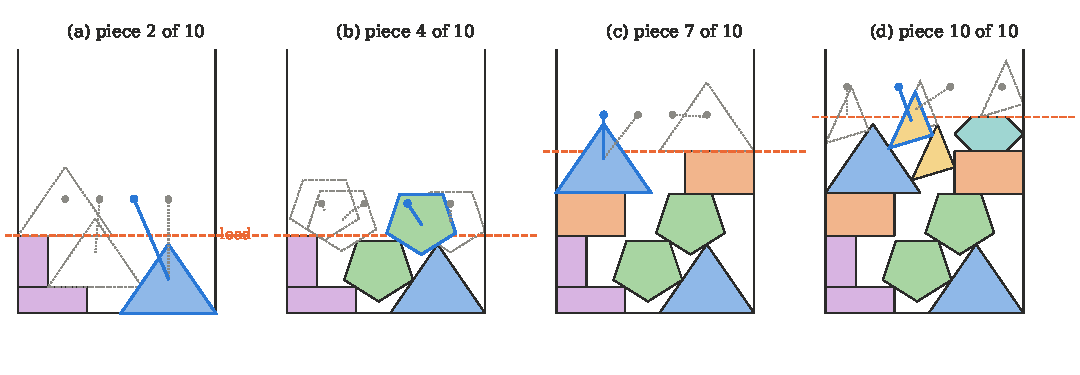
\includegraphics[width=\textwidth]{figures/construction.pdf}
\caption{Greedy construction on a 2D example (10 pieces, one of them a union of two convex parts), computed with a
2D version of the method. In each step, a piece starts from $g=4$ points on top of the current load (dots) and
descends by a sequence of LPs over NFP facets, towards the floor and the nearest wall; dotted outlines: final
positions of the other starts; blue: descent and position chosen by the greedy criterion.}
\label{fig:construction}
\end{figure}

\begin{figure}[!tbp]
\centering
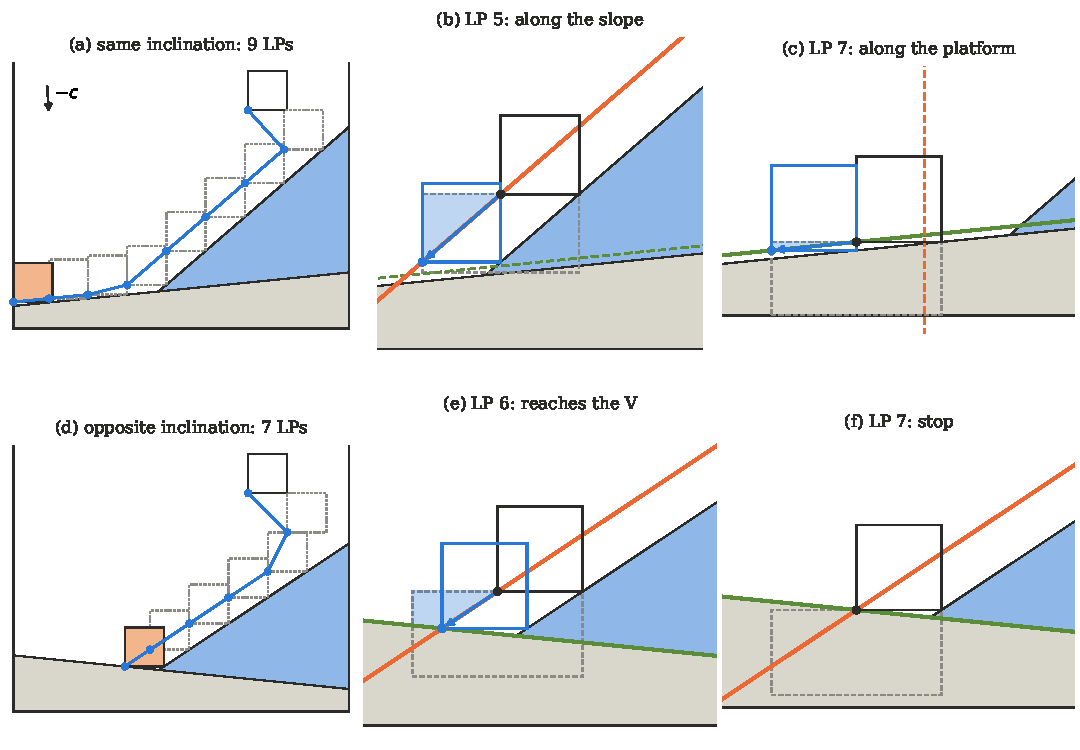
\includegraphics[width=\textwidth]{figures/descend.pdf}
\caption{\textsc{Descend} step by step on a 2D example: a square falls onto a slope that ends on a platform
whose top is slightly inclined, (a)--(c) in the same direction as the slope, (d)--(f) in the opposite direction.
(a), (d) The whole descent: each dot is the reference point of the square (the corner of its bounding box) after
one LP, and the dotted boxes are the trust regions. In free space the optimum of the LP is a corner of the trust
region, so the square moves down and towards the nearest wall; once it touches the slope it slides along it.
(b), (c), (e), (f) Single LPs (Algorithm~\ref{alg:greedy}, line~14) in the space of the reference point: $t$ is
the current point, the dashed box the trust region (the point may not go up), each line the facet selected for
a placed part (orange: slope; green: platform; solid if active at the optimum), the shaded region the feasible
region, and the arrow the move to the optimum along $-c$. (b) The square slides along the slope; the facet of the
platform is already selected but not active yet. (c) On the platform, the facet of the platform is active and
the square keeps sliding, down the slight incline, to the wall. (e) With the opposite inclination, the square
reaches the V between the slope and the platform. (f) Both facets are active and no direction decreases
$c\cdot t$: the descent stops. Gravity has priority over the wall term, so the piece slides down any incline.}
\label{fig:descend}
\end{figure}

\subsection{Global LP compaction}\label{sec:compact}
\textsc{Compact} is applied to feasible layouts: after the construction and after each successful separation.
It solves a sequence of linear programs over all translations. Given the current layout, for every
pair of parts that can touch within a trust region (each coordinate may move at most $\Delta$, half of the
smallest piece dimension) one NFP facet $f$ satisfied by the current relative position is selected and the
constraint $n_f\cdot(t_i-t_j)\ge d_f$ is imposed. The LP
\begin{equation}\label{eq:lp}
\begin{aligned}
\min\ & H+\epsilon\sum_i z_i\\
\text{s.t.}\ & z_i+h_i\le H,\quad \|t_i-t_i^0\|_\infty\le\Delta, && i=1,\dots,n,\\
& \text{container bounds on } t_i, && i=1,\dots,n,\\
& n_f\cdot(t_i-t_j)\ge d_f, && \text{selected pairs of parts},
\end{aligned}
\end{equation}
has a convex feasible region that contains the current layout. The facets are re-selected and the LP is
solved again while $H$ decreases. A solution is accepted only if it is feasible (the LP solution is checked for
bounds and overlap).

Algorithm~\ref{alg:compact} shows how the LP is used. \textsc{LPCompact} (lines~7--15) re-selects the facets
around each new layout, so that the pieces can slide along each other over several LPs, and stops when the height
no longer decreases. The facet chosen for a pair (line~10) is the one that lets the higher of the two pieces
descend the most with respect to the other. \textsc{Compact} alternates the LP with a local improvement
(\textsc{Improve}, lines~16--21) in which, from bottom to top, every piece descends again with the others fixed
(as in the greedy), and the pieces that define the height are moved to the lowest position generated as in
\textsc{Greedy}, if it is lower. The LP moves all pieces simultaneously but only within the trust region, while
\textsc{Improve} moves one piece at a time but can relocate it anywhere.

\begin{algorithm}[!htb]
\caption{Compaction of a feasible layout}\label{alg:compact}
\SetCommentSty{textit}
\Fn{\textsc{Compact}($T$)}{
  $T\gets$ \textsc{Improve}($T$)\;
  \Repeat{$H(T)$ does not decrease (at most 20 times)}{
    $T\gets$ \textsc{Improve}(\textsc{LPCompact}($T$))\;
  }
  \Return $T$\;
}
\Fn{\textsc{LPCompact}($T$)}{
  \Repeat{$H(T)$ does not decrease (at most 30 times)}{
    \ForEach{pair of parts $a\in\mathcal{A}_i$, $b\in\mathcal{A}_j$ that may meet in the trust region}{
      select the facet $f$ of $N_{ab}$ satisfied by $t_i-t_j$ that lets the higher piece descend the most\;
    }
    $T'\gets$ solution of LP~\eqref{eq:lp} with the selected facets\;
    \lIf{$T'$ violates a bound or overlaps (LP tolerances)}{\Return $T$}
    $T\gets T'$\;
  }
  \Return $T$\;
}
\Fn{\textsc{Improve}($T$)}{
  \ForEach{piece $i$ in increasing order of $z_i$}{
    $t_i\gets$ \textsc{Descend}($i,t_i,T\setminus\{i\}$)\tcp*{others fixed}
    \If{$z_i+h_i=H(T)$}{
      move $i$ to the lowest position generated as in \textsc{Greedy}, if it is lower\;
    }
  }
  \Return $T$\;
}
\end{algorithm}

\subsection{Strategic oscillation}
After a successful separation the target height is decreased by $\rho=1\%$ of the best height and the best
solution is clamped to it,
\begin{equation}
\textsc{Clamp}(T,h):\quad z_i\gets\min\{z_i,\ h-h_i\}\ \ (\text{and } x_i,y_i \text{ projected onto the
container}),\qquad i=1,\dots,n,
\end{equation}
which creates overlaps among the pieces near the top. After a failure the target is
increased by $\rho/4$ and the search continues from the overlapping layout, with the GLS weights of the previous
attempt. This scheme follows \citet{egeblad2009} and \citet{umetani2009}.

\subsection{Overlap minimization}\label{sec:minover}
\textsc{MinimizeOverlap} performs passes over the overlapping pieces in random order; for each piece the three
axes are tried in random order with the exact move of Proposition~\ref{prop:axis}. The pairwise penetrations are
kept in a matrix and only the row of a moved piece is recomputed. When a pass does not decrease~\eqref{eq:obj},
the GLS weights are updated multiplicatively as in \citet{gardeyn2025}: the weight of every overlapping pair is
multiplied by $1.2+0.8\,\delta_{ij}/\max\delta$, and the other weights decay by a factor $0.95$ (minimum 1). The
procedure stops when no overlap remains (then verified with a separating-axis test) or after 500 passes.
Weights persist along the oscillation and are reset after a successful separation or a restart.

In Algorithm~\ref{alg:minover}, line~2 computes the penetrations of all pairs, and each iteration of the loop is
a pass. Only the pieces involved in an overlapping pair are moved (line~7), each along the three axes with the
exact move of Proposition~\ref{prop:axis} (line~9), in which the weighted overlap $\phi$ of
Eq.~\eqref{eq:obj} is evaluated at the breakpoints and the best one is taken; since the current position is a
candidate, a move never increases $\phi$. After moving a piece, only its row of the penetration matrix is
recomputed (line~11). A pass without gain (line~12) is a local minimum of the weighted overlap; the weights of
the pairs that still overlap are then increased in proportion to their penetration, and those of the other pairs
decay, which changes $\phi$ and lets the next pass move the pieces out of the local minimum.

\begin{algorithm}[!htb]
\caption{Overlap minimization}\label{alg:minover}
\SetCommentSty{textit}
\Fn{\textsc{MinimizeOverlap}($T,h,w$)}{
  $P_{ij}\gets\delta_{ij}(t_i-t_j)$ for all pairs\tcp*{penetration matrix}
  \For{$\mathit{pass}=1,\dots,500$}{
    $O\gets\{(i,j):P_{ij}>0\}$\;
    \lIf{$O=\emptyset$}{\Return \KwSty{true} if the separating-axis test confirms it}
    $\mathit{gain}\gets 0$\;
    \ForEach{piece $i$ of a pair of $O$, in random order}{
      \ForEach{axis $k\in\{x,y,z\}$ in random order}{
        $s^*\gets\arg\min_{s\in\mathcal{B}}\phi(s)$ over the breakpoints $\mathcal{B}$ of Proposition~\ref{prop:axis},
        with the container $[0,W-w_i]\times[0,D-d_i]\times[0,h-h_i]$\;
        $\mathit{gain}\gets\mathit{gain}+\phi(t_{ik})-\phi(s^*)$; $t_{ik}\gets s^*$\;
      }
      recompute row $i$ of $P$\;
    }
    \If(\tcp*[f]{local minimum: GLS}){$\mathit{gain}=0$}{
      $w_{ij}\gets\max(1,\,0.95\,w_{ij})$ for $(i,j)\notin O$;\quad
      $w_{ij}\gets w_{ij}\,(1.2+0.8\,P_{ij}/\max_O P)$ for $(i,j)\in O$\;
    }
  }
  \Return \KwSty{false}\;
}
\end{algorithm}

Figure~\ref{fig:passes} shows all the passes on the 2D example, from a clamped layout, followed by the LP
compaction.

\begin{figure}[!tbp]
\centering
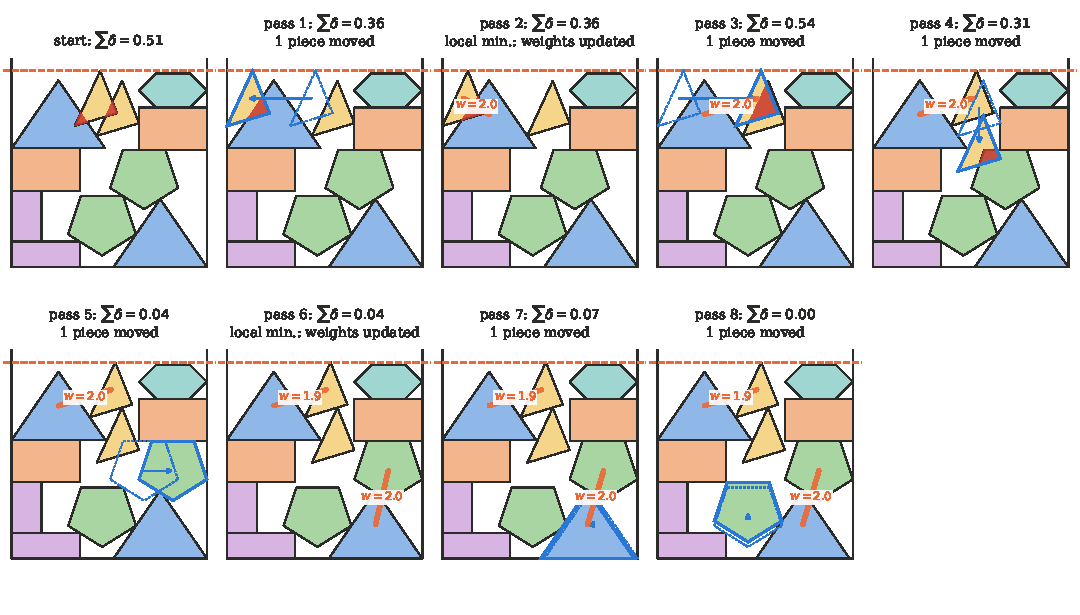
\includegraphics[width=\textwidth]{figures/passes.pdf}
\caption{\textsc{MinimizeOverlap} on the 2D example: the greedy layout of Figure~\ref{fig:construction} is clamped
to the target height $h=0.9H$ (dashed line), and every pass is shown. In each pass, the pieces
that overlap are moved along the axes; the pieces actually moved are outlined in blue (dashed: position before
the pass), and overlaps are in red. Each title
gives the unweighted overlap $\sum\delta$ and the weighted overlap $\sum w\delta$, which is the one minimized:
no move increases it. Pass~2 does not reduce it (a local minimum), so the weight of the overlapping pair of
triangles is increased from 1 to 2 and $\sum w\delta$ jumps from 0.36 to 0.71; the weights change the objective,
not the layout, and the next pass starts from the same positions. Pass~3 then moves the small triangle onto
the other one: $\sum w\delta$ decreases to 0.54, although $\sum\delta$ increases. The triangle is moved down in
pass~4. The same happens with the pentagon and the triangle at the bottom in passes~6--8, and after pass~8 the
layout is feasible. The last panel shows the LP compaction that follows (gray: before), which moves all pieces
simultaneously and lowers the height below $h$.}
\label{fig:passes}
\end{figure}

\subsection{Restarts}\label{sec:kicks}
When the target reaches the best height, the search restarts from the best solution clamped to $(1-\rho)H$, with
the weights reset, after moving one random piece (a kick): to a random position or, with probability 1/2, to the
lowest of the positions generated as in the greedy construction. On the larger instances the kick itself has no
measurable effect (Table~\ref{tab:ablation}): the diversification comes from the restart, with reset weights and
a new random order of the moves. The random positions are needed on small instances: with two pieces there is a
single pair, so the weights have no effect, and the search keeps returning to the layout produced by the greedy
order (Section~\ref{sec:t2025}).

% =====================================================================================================
\section{Computational experiments}\label{sec:exp}

\subsection{Setting}
The method is implemented in C++ on top of the Metasolver framework; LPs are solved with SoPlex 8.1
\citep{wunderling1996}. Experiments ran on two Intel Xeon E5-2620 v4 processors (2.1~GHz, 3.0~GHz turbo, 16 cores, 64~GB, Ubuntu 24.04,
g++ 13.3), one thread per run, 14 runs in parallel. Each configuration was run with 10 seeds and a time limit of 120 s per
instance. All reported solutions were verified with an independent checker that tests every pair of convex parts
for a separating axis.

\paragraph{Instances}
We use the 3D instances of the ESICUP repository \citep{esicup}:
\begin{itemize}
\item \emph{Stoyan 2005}, Examples 1--3 (7, 12 and 25 convex pieces) \citep{stoyan2005}. In the public data, one
piece (polytope7) has faces that use only 9 of its 10 vertices; we use its convex hull (volume 192.5), which
matches the volume reported by \citet{egeblad2009}.
\item \emph{Stoyan 2004}, Examples 1--5 (20--50 non-convex pieces) \citep{stoyan2004}, each defined as a union of
convex polytopes, which we use directly as the decomposition.
\item \emph{Merged1--5} \citep{egeblad2009}: $i$ copies of 15 pieces, the 7 convex pieces of Stoyan 2005 and the
8 pieces of \citet{ikonen1997} scaled by 4, in a container whose base is such that a layout with 50\%
utilization is a cube. Six Ikonen pieces are non-convex prisms; we decompose them exactly by triangulating the
base polygon, merging triangles into convex polygons \citep{hertel1983}, and extruding (a frame is split into
four boxes; two pieces have polygons touching at a vertex). The volumes of the parts match those of the meshes.
\item \emph{Liu Experiment 1} \citep{liu2015}: 36 pieces (8 tetrahedra, 8 cubes, 8 stars, 8 arrows and 4 rings)
in a $20\times20$ container; the stars, arrows and rings are prisms and are decomposed exactly in the same way.
\end{itemize}

\paragraph{References}
3DNest \citep{egeblad2009} uses the same exact geometry; its average and maximum utilization over 10 runs of
600 s (one core of a 2.16~GHz Core Duo) are converted to heights. \citet{lamas2023} report best and average heights
of a voxel VNS; their voxelization overestimates the pieces (by 15\% in volume for Merged1, as they note), so
their heights are not directly comparable. For Stoyan 2004 the only exact reference is \citet{stoyan2004}.

\subsection{Component analysis}
Table~\ref{tab:ablation} evaluates the components on the seven hardest instances (Stoyan 2004 Examples 1--5 and
Stoyan 2005 Examples 2--3). Each row changes one element of the method. The effect of the speed of the separation
is estimated by stopping the same runs at 24 s, which corresponds to moves five times slower.

The multiplicative weights and the speed of the separation are the decisive elements: with additive weights the
mean heights increase on Stoyan 2004 Examples 3--5 and Stoyan 2005 Example 3 (e.g., from 53.60 to 55.27 on
Stoyan 2004 Example 4), and five times slower moves lose most of the advantage. The kick has no measurable effect
on these instances: all the variants in the lower part of the table, including restarting from the best solution
without moving any piece, give the same results within one or two standard errors. A top piece is one that
exceeds the target height; moving it to the least overlapped of 20 random positions gives a slightly lower mean
on Stoyan 2004 Example 1 but not on the others. The diversification thus comes mainly from the restart itself,
with reset weights and a new random order of the moves. The random moves are needed only on small instances
(Section~\ref{sec:t2025}). The LP compaction has no significant effect: the
differences are of about one standard error, slightly in favour of the variant without LP on Stoyan 2004. It is therefore not needed for the quality of the solutions, and
the method can run without an LP solver.

\begin{table}[t]
\centering\small
\caption{Mean gap of the height with respect to the best published value (Stoyan 2004 Examples 2--5 and Stoyan
2005 Examples 2--3) and mean height on Stoyan 2004 Example 1 (no published reference); 120 s, mean of 10 seeds.
Negative is better.}\label{tab:ablation}
\begin{tabular}{p{0.45\textwidth}rrr}
\toprule
Configuration & Stoyan 2004 & Stoyan 2005 & S2004 Ex1\\
\midrule
Proposed method & $-2.8\%$ & $-2.0\%$ & 53.41\\
Without LP compaction & $-3.3\%$ & $-1.9\%$ & 53.30\\
Additive GLS weights ($w_{ij}\gets w_{ij}+1$) & $-1.3\%$ & $-1.5\%$ & 53.15\\
Separation five times slower (runs stopped at 24 s) & $-0.1\%$ & $-0.9\%$ & 54.82\\
\midrule
Kick: reinsertion only & $-3.5\%$ & $-1.9\%$ & 53.50\\
Kick: random position only & $-3.1\%$ & $-1.9\%$ & 53.60\\
Kick: a top piece to a random position & $-3.0\%$ & $-1.9\%$ & 53.16\\
Kick: a top piece to the least overlapped of 20 random positions & $-2.8\%$ & $-2.1\%$ & 53.09\\
No kick (restart from the best solution only) & $-2.8\%$ & $-2.0\%$ & 53.66\\
\bottomrule
\end{tabular}
\end{table}

\subsection{Comparison with the literature}
Table~\ref{tab:results} compares the method with the literature. On the instances that share the exact
geometry of 3DNest (Stoyan 2005 Examples 2--3 and Merged1--5), the method obtains lower heights in six of seven
cases; the exception is Stoyan 2005 Example 2 (19.13 versus 19.01). The improvement grows with the size of the
instance: on Merged3--5 our best heights are 8--10\% below the best known values, obtained by the voxel VNS
with the finest resolution and four hours, and our mean heights after 120 s are lower than those best values. On Stoyan 2004, the method improves the exact reference by
a wide margin, and on Example 2 it reaches the optimum.

\begin{table}[t]
\centering\small
\caption{Heights (lower is better). Exact: 3DNest \citep{egeblad2009} (best and mean of 10 runs of 600 s),
optimum of \citet{tollenaere2026} for Stoyan 2005 Example 1, and \citet{stoyan2004} (St04). Voxels: VNS of
\citet{lamas2023} (best: standard resolution and 10 runs of 1 h for Stoyan, extra-fine resolution and 4 h for
Merged; mean: standard resolution). Ours: mean (best) of 10 seeds, 120 s. $^*$Optimal (equal to the lower bound
$H_0$). $^\dagger$Value reported by \citet{lamas2023}; it is below the height of the tallest piece (29) in the
public data. $^\ddagger$HAPE3D \citep{liu2015}, allowing 8 rotations. $^\S$Not exact: conservative convex decomposition
(Section~\ref{sec:exp}, Discussion); ours: 5 seeds of 20 min (15 min with a coarse decomposition and 5 min with a
fine one); voxels: 10 runs of 1 h.}
\label{tab:results}
\begin{tabular}{lrrrrrr}
\toprule
& & \multicolumn{2}{c}{Exact} & \multicolumn{2}{c}{Voxels} & \\
\cmidrule(lr){3-4}\cmidrule(lr){5-6}
Instance & $n$ & best & mean & best & mean & Ours\\
\midrule
Stoyan 2005 Ex1 & 7 & 17.46 (opt.) & -- & -- & -- & 17.47 (17.46)\\
Stoyan 2005 Ex2 & 12 & \textbf{19.01} & 19.83 & 21.23 & 21.70 & 19.13 (19.13)\\
Stoyan 2005 Ex3 & 25 & 28.83 & 29.82 & 29.76 & 31.53 & \textbf{27.50 (27.22)}\\
Stoyan 2004 Ex2 & 20 & 32 (St04) & -- & 28.47$^\dagger$ & 29.40 & \textbf{29.00 (29.00)}$^*$\\
Stoyan 2004 Ex3 & 30 & 49 (St04) & -- & 41.30 & 42.65 & \textbf{39.90 (39.00)}\\
Stoyan 2004 Ex4 & 40 & 63.21 (St04) & -- & 54.83 & 59.52 & \textbf{53.60 (52.35)}\\
Stoyan 2004 Ex5 & 50 & 78.7 (St04) & -- & 72.33 & 76.81 & \textbf{66.81 (64.97)}\\
Merged1 & 15 & 17.00 & 17.45 & 17.13 & 18.67 & \textbf{16.54 (16.04)}\\
Merged2 & 30 & 21.98 & 22.02 & 22.06 & 22.64 & \textbf{21.04 (21.00)}\\
Merged3 & 45 & 24.04 & 24.97 & 24.32 & 26.26 & \textbf{22.53 (22.02)}\\
Merged4 & 60 & 27.81 & 28.35 & 26.47 & 29.44 & \textbf{25.31 (24.40)}\\
Merged5 & 75 & 30.13 & 31.31 & 29.24 & 31.12 & \textbf{27.88 (26.44)}\\
Liu Exp.~1 & 36 & 31.2$^\ddagger$ & -- & 34.27 & 35.37 & \textbf{30.11 (29.52)}\\
\midrule
\multicolumn{7}{l}{\emph{Curved meshes (conservative decomposition)}}\\
Chess$^\S$ & 32 & -- & -- & \textbf{131} & \textbf{135.1} & 145.0 (139.2)\\
\bottomrule
\end{tabular}
\end{table}

On Stoyan 2004 Example 2 our height, 29, equals the lower bound $H_0$ given by the tallest piece, so it is
optimal for the public data. Stoyan 2004 Example 1 (80 pieces) has no published reference and is not included;
the instance called Experiment 1 by \citet{lamas2023} is the one of \citet{liu2015}, where our mean height is
12\% below the best voxel height and also below that of HAPE3D, which allows rotations. For Stoyan 2005 Example 1, the utilization reported by \citet{egeblad2009} converts to
a height below the proven optimum with our data, so the instance seems to differ and we only compare with the
optimum. Figure~\ref{fig:solutions} shows two of the best solutions.

\begin{figure}[!tbp]
\centering
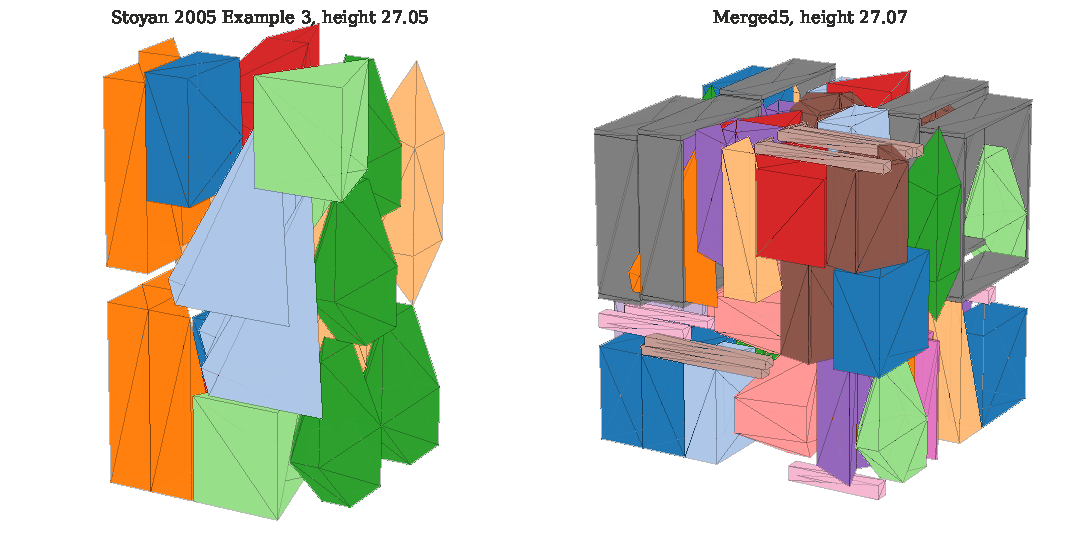
\includegraphics[width=\textwidth]{figures/solutions.pdf}
\caption{Best solutions of the final runs for Stoyan 2005 Example 3 and Merged5.}\label{fig:solutions}
\end{figure}

\subsection{Comparison with exact models}\label{sec:t2025}
\citet{tollenaere2026} solve four series of small instances (2--20 items of the convex pieces of Stoyan 2005 and
Stoyan 2004, of diamonds and of tetrahedra) with mixed-integer models based on no-fit polyhedra, with a time limit
of one hour per model; they prove optimality for 27 of the 66 instances and report upper and lower bounds for the
others. Table~\ref{tab:t2025} summarizes our results (10 seeds, 30 s per instance). The method finds 26 of the 27
proven optima in its best run, 20 of them in every run; the exception is the 10-item instance of the Stoyan 2005
series (26.20 versus 26.05). On the 39 open instances it improves the best upper bound in 32 cases, by 5\% on
average, and matches it in most of the others. Before adding random moves to the restarts, the method missed the
optimum of two 2-item instances (by 17\% and 28\%): the greedy places the larger piece on the floor, the optimum
needs the opposite arrangement, and neither the GLS weights (a single pair) nor reinsertion could escape.

\begin{table}[t]
\centering\small
\caption{Instances of \citet{tollenaere2026} (10 seeds, 30 s). Optima: instances with proven optimum, and number
of them found in the best run and in all runs. Open: instances without proven optimum, number in which our best
height is below the best upper bound of the models, and mean gap of our mean height with respect to that bound.}
\label{tab:t2025}
\begin{tabular}{lrrrrrr}
\toprule
& & \multicolumn{3}{c}{Optima} & \multicolumn{2}{c}{Open}\\
\cmidrule(lr){3-5}\cmidrule(lr){6-7}
Series & $n$ & proven & best run & all runs & improved & gap\\
\midrule
Diamonds & 9 & 4 & 4 & 2 & 5 of 5 & $-4.5\%$\\
Stoyan 2004 & 19 & 9 & 9 & 6 & 9 of 10 & $-5.0\%$\\
Stoyan 2005 & 19 & 9 & 8 & 7 & 9 of 10 & $-4.7\%$\\
Tetrahedra & 19 & 5 & 5 & 5 & 9 of 14 & $-1.7\%$\\
\midrule
Total & 66 & 27 & 26 & 20 & 32 of 39 & \\
\bottomrule
\end{tabular}
\end{table}

\subsection{Time-matched comparison}
Hardware differs by about ten years. Figure~\ref{fig:time} compares the mean utilization over time with that
of 3DNest at 10, 60, 300 and 600 seconds. Our first solution is available after about 0.3 seconds (the
greedy construction and compaction), and at 10 seconds our mean utilization already exceeds the mean utilization
of 3DNest at 600 seconds on all five instances (44.3, 43.4, 45.1, 44.7 and 43.2\% versus 43.0, 42.9, 43.3, 42.0
and 41.0\%). Even assuming that our machine is five times faster per core, the
advantage holds at equal effective time.

\begin{figure}[!tbp]
\centering
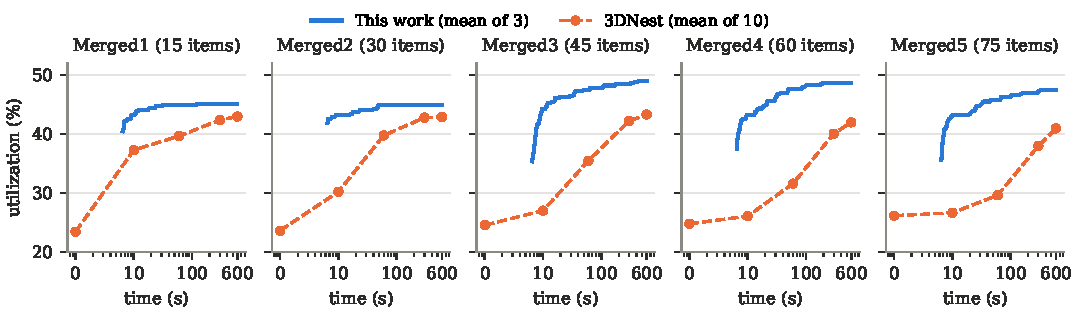
\includegraphics[width=\textwidth]{figures/merged_time.pdf}
\caption{Mean utilization over time on the Merged instances (10 seeds), compared with 3DNest
\citep[Table 3]{egeblad2009} (10 runs).}
\label{fig:time}
\end{figure}

\subsection{Discussion}
The results support a conclusion that agrees with recent 2D work \citep{gardeyn2025}: the quality of an
overlap-minimization heuristic is driven by how many separation attempts fit in the time budget, and therefore
by the cost of evaluating and optimizing the overlap. The NFP-based penetration depth gives an exact, cheap and
informative measure for unions of convex parts with few facets, which is the case of all the benchmark
instances.

\paragraph{Realistic meshes}
The cost of a move grows with the number of facets of the NFPs, so pieces with curved surfaces are the hard case.
We tested the Chess instance of \citet{lamas2023} (32 pieces, meshes of 700--2900 triangles). Since an exact
convex decomposition of such meshes is impractical, we use a conservative one (the large convex hulls of the NFPs are computed with Qhull \citep{barber1996}): CoACD \citep{wei2022} cuts the
mesh and takes the convex hull of each piece; the small gaps it leaves between parts are covered by scaling
each part from its centroid, and containment is checked with interior sample points. With concavity threshold
0.05 (6--20 parts per piece) the union exceeds the volume of the piece by 4--12\%, and with 0.2 (1--4 parts,
reduced to at most 42 facet directions) by 38--78\%. The solutions remain feasible for the real geometry.
However, the NFPs between parts have hundreds of facets and a separation takes 20--35 s instead of a fraction of
a second. In 20 minutes (5 seeds; Table~\ref{tab:results}) the best (mean) heights are 143.6 (150.5) with the fine decomposition, 151.2 (152.5) with
the coarse one and 139.2 (145.0) with 15 minutes of coarse search followed by 5 minutes of refinement with the
fine decomposition, against 131 (best of 10 runs of 1 h) and 135.1 (mean) for
the voxel VNS of \citet{lamas2023}, whose cost does not depend on the complexity of the surface. Pseudo-blocks of
two pieces did not help. The other realistic instance of \citet{lamas2023}, Engine (97 pieces with meshes of up to
342{,}000 triangles), was not tested, for the same reason. Voxels and the proposed method are thus complementary: the latter is faster and exact
on polyhedral pieces with few facets, the former scales better to curved meshes.

\paragraph{Limitations}
Rotations are not considered. The method requires a convex decomposition of each piece; for the benchmark
instances it is exact and small, while for curved meshes a conservative decomposition overestimates the pieces
and, above all, makes the moves expensive. Reducing the cost of the NFPs of curved parts (e.g., hierarchical
filtering with the hull of each piece, or conservative simplification of the NFPs) is left for future work.

% =====================================================================================================
\section{Conclusions}
We presented an overlap-minimization heuristic for 3D irregular strip packing that works with the exact geometry
of polyhedra given as unions of convex parts. Its key element is an exact axis move based on penetration depths
in no-fit polytopes, combined with multiplicative guided local search, strategic oscillation and restarts. This simple method outperforms
the previous methods, with exact and voxel geometry, on the benchmarks of polyhedral pieces, and matches almost
all the proven optima of the small instances. On curved meshes, which require conservative decompositions with
many facets, it remains behind voxel-based search. Future work includes cheaper NFP computations for curved
parts, rotations, larger instances from additive manufacturing, and lower bounds.

\bibliographystyle{elsarticle-harv}
\bibliography{refs}

\end{document}
